\documentclass[10pt]{beamer}
% 8pt, 9pt, 10pt, 11pt, 12pt, 14pt, 17pt and 20pt.
% Choose how your presentation looks.
%
% For more themes, color themes and font themes, see:
% http://deic.uab.es/~iblanes/beamer_gallery/index_by_theme.html
%
\mode<presentation>
{
%  \usetheme{Berlin}      % or try Darmstadt, Madrid, Warsaw, ...
	\usetheme[
		bullet=circle,                  % Use circles instead of squares for bullets
		titleline=false,                % Show a line below the frame
		alternativetitlepage=true,      % Use the fancy title
		titlepagelogo=logo-sapienza,    % Logo for the first slide
		watermark=watermark-sapienza,   % Watermark used in every slide
		watermarkheight=20px,           % Desired height of the watermark
		watermarkheightmult=6,          % Watermark image is actually x times bigger
		displayauthoronfooter=true		
	]{Roma}
%  \usecolortheme{beaver} % or try albatross, beaver, crane, ...
%  \usefonttheme{default}  % or try serif, structurebold, ...
  %\setbeamertemplate{navigation symbols}{}
% \setbeamertemplate{caption}[numbered]
} 

\usepackage[english]{babel}
\usepackage[utf8x]{inputenc}
\makeatletter
\let\@@magyar@captionfix\relax
\makeatother
%other packages...
\usepackage{hyperref}
\usepackage{xspace}
\usepackage{tabularx} % in the preamble
\usepackage{subfigure}
%\usepackage{subfig}
%\usepackage{chngcntr}
%\counterwithin{subfigure}{figure}
% The algorithm packages have to be after hyperref.
\usepackage{algorithm}
\usepackage{algpseudocode}
\usepackage{multirow}
\usepackage{animate}
\usepackage{tasks}

\usepackage{adjustbox}
\usepackage{multimedia}
%\usepackage{movie15}


\usepackage{tikz}
\usetikzlibrary{arrows}
% For every picture that defines or uses external nodes, you'll have to
% apply the 'remember picture' style. To avoid some typing, we'll apply
% the style to all pictures.
\tikzstyle{every picture}+=[remember picture]

% By default all math in TikZ nodes are set in inline mode. Change this to
% displaystyle so that we don't get small fractions.
\everymath{\displaystyle}
\tikzstyle{na} = [baseline=-.5ex]


%%%%%%%%%%%%%%%%%%%%%%%%%% General
\newcommand{\Section}[1]{Section \ref{#1}}

\newcommand{\myi}{(\emph{i})\xspace}
\newcommand{\myii}{(\emph{ii})\xspace}
\newcommand{\myiii}{(\emph{iii})\xspace}
\newcommand{\myiv}{(\emph{iv})\xspace}
\newcommand{\myv}{(\emph{v})\xspace}
\newcommand{\myvi}{(\emph{vi})\xspace}
\newcommand{\myvii}{(\emph{vii})\xspace}
\newcommand{\myviii}{(\emph{viii})\xspace}

%% general math
%\newcommand{\A}{\mathcal{A}} 
\newcommand{\B}{\mathcal{B}}
%\newcommand{\C}{\mathcal{C}} 
\newcommand{\D}{\mathcal{D}}
\newcommand{\E}{\mathcal{E}} \newcommand{\F}{\mathcal{F}}
\newcommand{\G}{\mathcal{G}} \renewcommand{\H}{\mathcal{H}}
\newcommand{\I}{\mathcal{I}} \newcommand{\J}{\mathcal{J}}
\newcommand{\K}{\mathcal{K}} \renewcommand{\L}{\mathcal{L}}
\newcommand{\M}{\mathcal{M}} \newcommand{\N}{\mathcal{N}}
\renewcommand{\O}{\mathcal{O}} \renewcommand{\P}{\mathcal{P}}
\newcommand{\Q}{\mathcal{Q}} \newcommand{\R}{\mathcal{R}}
\renewcommand{\S}{\mathcal{S}} \newcommand{\T}{\mathcal{T}}
\newcommand{\U}{\mathcal{U}} \newcommand{\V}{\mathcal{V}}
\newcommand{\W}{\mathcal{W}} \newcommand{\X}{\mathcal{X}}
\newcommand{\Y}{\mathcal{Y}} \newcommand{\Z}{\mathcal{Z}}

\newcommand{\limp}{\mathbin{\rightarrow}}
\newcommand{\ind}{\hspace*{.18in}}

\newcommand{\cla}[1]{\makebox[0pt]{\hss#1\hss}}
\newcommand{\Once}{%
  \sbox0{$\Diamond$}%
  \usebox0\kern-.5\wd0\cla{\raisebox{.1ex}{\scalebox{.7}[1]{$-$}}}\kern.5\wd0%
}

%% LTL
\newcommand{\Atom}{A}
\newcommand{\Always}{\raisebox{-0.27ex}{$\square$}}
\newcommand{\Next}{\raisebox{-0.27ex}{\LARGE$\circ$}}
\newcommand{\Wnext}{\raisebox{-0.27ex}{\LARGE$\bullet$}}
\newcommand{\lUntil}{\mathop{\U}}
\newcommand{\Yesterday}{\raisebox{-0.27ex}{$\ominus$}}
\newcommand{\Since}{\mathop{\S}}
\newcommand{\Release}{\mathop{\R}}
\newcommand{\Wuntil}{\mathop{\W}}
\newcommand{\true}{\mathit{true}}
\newcommand{\final}{\mathit{Final}}
\newcommand{\false}{\mathit{false}}
\newcommand{\ttrue}{{\mathit{tt}}}
\newcommand{\ffalse}{\mathit{ff}}
\newcommand{\Last}{\mathit{Last}}
\newcommand{\Ended}{\mathit{End}}
\newcommand{\length}{\mathit{length}}
\newcommand{\last}{\mathit{last}}
\newcommand{\End}{\mathit{end}}
\newcommand{\nnf}{\mathit{nnf}}
\newcommand{\BOX}[1]{ [#1]}
\newcommand{\DIAM}[1]{\langle #1 \rangle}
\newcommand{\transl}{f}


%% Logics
\newcommand{\LT}{{\sc lt}$_f$\xspace}
\newcommand{\LTi}{{\sc lt}$_i$\xspace}
\newcommand{\PLTL}{{\sc pltl}\xspace}
\newcommand{\FLTL}{{\sc \$fltl}\xspace}
\newcommand{\FstarLTL}{{\sc \$$^*$fltl}\xspace}
\newcommand{\PL}{{\sc pl}\xspace}
\newcommand{\LTL}{{\sc ltl}\xspace}
\newcommand{\LTLf}{{\sc ltl}$_f$\xspace}
\newcommand{\PLTLf}{{\sc pltl}$_f$\xspace}
\newcommand{\LTLp}{{\sc ltl}p$_f$\xspace}
\newcommand{\LDL}{{\sc ldl}\xspace}
\newcommand{\LDLf}{{\sc ldl}$_f$\xspace}
\newcommand{\RE}{{\sc re}$_f$\xspace}
\newcommand{\REGEX}{{\sc re}\xspace}
\newcommand{\DL}{{\sc dl}\xspace}
\newcommand{\PDL}{{\sc pdl}\xspace}
\newcommand{\PDDL}{{\sc pddl}\xspace}
\newcommand{\FOND}{{\sc fond}\xspace}
\newcommand{\FOf}{{\sc fo}$_f$\xspace}
\newcommand{\MSOf}{{\sc mso}$_f$\xspace}
\newcommand{\FO}{{\sc fo}\xspace}
\newcommand{\FOL}{{\sc fol}\xspace}
\newcommand{\MSO}{{\sc mso}\xspace}
%\newcommand{\ATA}{{\sc ata}\xspace}
\newcommand{\AFW}{{\sc afw}\xspace}
\newcommand{\NFA}{{\sc nfa}\xspace}
\newcommand{\DFA}{{\sc dfa}\xspace}
\newcommand{\DFAs}{{\sc dfa}s\xspace}
\newcommand{\GTAs}{{\sc gta}s\xspace}
\newcommand{\declare}{{\sc declare}\xspace}
\newcommand{\wsos}{{\sc ws1s}\xspace}
\newcommand{\wsts}{{\sc ws2s}\xspace}
\newcommand{\bdds}{{\sc bdd}s\xspace}
\newcommand{\bdd}{{\sc bdd}\xspace}
\newcommand{\mls}{{\sc m2l-s}tr\xspace}
\newcommand{\fol}{\mathit{fol}}
\newcommand{\folp}{\mathit{fol_p}}
\newcommand{\f}{\mathit{f}}
%\newcommand{\g}{\mathit{g}}
\newcommand{\re}{\mathit{re}}


\newcommand{\tup}[1]{\langle #1 \rangle}

\newcommand{\Stop}{\mathit{stop}}
\newcommand{\rew}{\mathit{rew}}
\newcommand{\Tr}{\mathit{Tr}}

\newcommand{\LOGSPACE}{{\sc logspace}\xspace}
\newcommand{\NLOGSPACE}{{\sc nlogspace}\xspace}
\newcommand{\PTIME}{{\sc ptime}\xspace}
\newcommand{\NP}{{\sc np}\xspace}
\newcommand{\EXPTIME}{{\sc exptime}\xspace}
\newcommand{\PSPACE}{{\sc pspace}\xspace}
\newcommand{\TWOEXPTIME}{{\sc 2exptime}\xspace}


\newcommand{\expand}{\textbf{\textit{E}}}
\newcommand{\ttt}{{\textbf{\textit{T}}}}
\newcommand{\fff}{{\textbf{\textit{\texttt{F}}}}}

\newcommand{\fstate}{s_f}

\newcommand{\atomize}[1]{\texttt{"}\ensuremath{#1}\texttt{"}}


% misc
\newcommand{\MONA}{{\sc mona}\xspace}
\newcommand{\FLLOAT}{{\sc flloat}\xspace}
\newcommand{\suc}{\textit{succ}\xspace}
\newcommand{\pre}{\textit{prev}\xspace}
\newcommand{\folInter}{$\I = (\Delta^I,\cdot^{\I})$\xspace}
\newcommand{\rcon}{RCon}
\newcommand{\janus}{{\sc janus}\xspace}

%RL
\newcommand{\MDP}{\M}
\newcommand{\States}{S}
\newcommand{\Actions}{A}
\newcommand{\TrFun}{T}
\newcommand{\Reward}{R}
\newcommand{\DiscFact}{\gamma}
\newcommand{\Policy}{\rho}
\newcommand{\ExpRet}{G}
\newcommand{\ValFun}{v}
\newcommand{\qFun}{q}

\newcommand{\ValOptFun}{\ValFun^*}
\newcommand{\qOptFun}{\qFun^*}
\newcommand{\OptPolicy}{\Policy^*}

\newcommand{\ValFunEst}{V}
\newcommand{\qFunEst}{Q}
\newcommand{\LRate}{\alpha}

\newcommand{\NMRDP}{\N}
\newcommand{\NMReward}{\bar{\Reward}}
\newcommand{\NMPolicy}{\bar{\Policy}}

\newcommand{\traj}{\tup{s_0, a_0, \dots, s_{n-1}, a_{n-1}, s_n}}
\newcommand{\trajprime}{\tup{s'_0, a_0, \dots, s'_{n-1}, a_{n-1}, s'_n}}
\newcommand{\projtraj}{\tup{s_0, s_1, \dots, s_n}}
\newcommand{\projtrajprime}{\tup{s'_0, s'_1, \dots, s'_n}}

\newcommand{\MDPagent}{\MDP_{ag}}
\newcommand{\TrFunAgentGoal}{\TrFun_{ag}^{g}}

\newcommand{\bqs}{\mathbf{q}}

%LOGIC

\newcommand{\Prop}{\P}
\newcommand{\PropInt}{\Pi}
\newcommand{\PropFormula}{\phi}
\newcommand{\trace}{\pi}
\newcommand{\Kripke}{\K}
\newcommand{\tm}[1]{\ \text{#1}\ }
\newcommand{\tiff}{\tm{iff}}
\newcommand{\DECLARE}{{\sc declare}\xspace}


\newcommand{\automaton}{\mathcal{A}}
\newcommand{\LLf}{\LTLf/\LDLf}
\newcommand{\DfunSym}{\partial}
\newcommand{\Dfun}[1]{\DfunSym\lparen #1,\PropInt \rparen}
\newcommand{\DfunEps}[1]{\DfunSym\lparen #1, \epsilon\rparen}
\newcommand{\lAND}{\wedge}
\newcommand{\lOR}{\vee}
\newcommand{\NOT}{\lnot}
\newcommand{\regexp}{\varrho}
\newcommand{\TrueDelta}[1]{\textit{\textbf{\texttt{T}}}_{#1}}
\newcommand{\FalseDelta}[1]{\textit{\textbf{\texttt{F}}}_{#1}}
\newcommand{\bOne}{\mathbf{1}}
\newcommand{\bZero}{\mathbf{0}}
\newcommand{\LTS}{{\sc lts}\xspace}
\newcommand{\LDLfToNFA}{{\sc ldl}$_f2$\NFA}
\newcommand{\LDLfToDFA}{{\sc ldl}$_f2$\DFA}
\newcommand{\LTLfToDFA}{{\sc ltl}$_f2$\DFA}
\newcommand{\PLTLToDFA}{{\sc pltl}$2$\DFA}
\newcommand{\LTLfToFOL}{{\sc ltl}$_f2$\FOL}
\newcommand{\PLTLToFOL}{{\sc pltl}$2$\FOL}

\newcommand{\Sapientino}{{\sc sapientino}\xspace}
\newcommand{\Breakout}{{\sc breakout}\xspace}
\newcommand{\Minecraft}{{\sc minecraft}\xspace}

%math

\newcommand{\set}[1]{\{#1\}}
\newcommand{\Naturals}{\mathbb{N}}
\newcommand{\Reals}{\mathbb{R}}
\newcommand{\defeq}{\coloneqq}


%algpseudocode
\algnewcommand\algInput{\textbf{input}}
\algnewcommand\algOutput{\textbf{output}}


%%% Local Variables:
%%% mode: latex
%%% TeX-master: "main"
%%% save-place: t
%%% End:



\usepackage{listings}
% Custom colors
\usepackage{color}
\definecolor{deepblue}{rgb}{0,0,0.5}
\definecolor{deepred}{rgb}{0.6,0,0}
\definecolor{deepgreen}{rgb}{0,0.5,0}
\definecolor{backcolour}{rgb}{0.95,0.95,0.92}
\definecolor{codegray}{rgb}{0.5,0.5,0.5}

\usepackage{accsupp}    
\newcommand{\noncopynumber}[1]{
	\BeginAccSupp{method=escape,ActualText={}}
	#1
	\EndAccSupp{}
}
\lstdefinestyle{Python}{
	language        = Python,
	backgroundcolor=\color{backcolour},
	basicstyle      = \small\ttfamily,
	keywordstyle    = \color{deepblue},
	stringstyle     = \color{deepgreen},
	commentstyle    = \color{codegray}\ttfamily,
	numberstyle=\tiny\color{codegray}\noncopynumber,
	columns=flexible,
	numbers=left,
	stepnumber=1
}

\ifodd\textwidth
\addtolength{\textwidth}{1sp}
\fi


\title[\LTLf and \PLTL for Planning and Declarative Process Mining]{\LTL and Past \LTL on Finite Traces for Planning and Declarative Process Mining}
\author{Francesco Fuggitti}
\institute[DIAG at Sapienza, Rome]{Master of Science in \\Engineering in Computer Science\\ Sapienza, University of Rome\\ \bigskip \scriptsize Advisor: Prof. Giuseppe De Giacomo}
\date{\scriptsize A.Y. 2017/2018}
%Advisor: prof. Giuseppe De Giacomo

\newcounter{saveenumi}
\newcommand{\seti}{\setcounter{saveenumi}{\value{enumi}}}
\newcommand{\conti}{\setcounter{enumi}{\value{saveenumi}}}

\resetcounteronoverlays{saveenumi}

\begin{document}

\begin{frame}[t, plain]
  \titlepage
\end{frame}

% Uncomment these lines for an automatically generated outline.
\begin{frame}{Outline}
  \tableofcontents
\end{frame}


\section{Introduction}
\begin{frame}{Introduction}
\begin{itemize}
	\item \textit{Linear Temporal Logic} (\LTL) is a simple formal language for expressing temporal specifications both in Artificial Intelligence (AI) and in Business Process Management (BPM)
	\begin{itemize}
	\item \LTL on \emph{finite} traces (\LTLf) (De Giacomo and Vardi, 2013)
	\item Past \LTL on \emph{finite} traces (\PLTL) (Lichtenstein et al. 1985)
	\end{itemize}
	
	\vskip 0.5cm
	\item In AI: planning for temporally extended goals from Bacchus and Kabanza, (1998) to
	Camacho et al. (2017/2018)
	
	\vskip 0.5cm
	\item In BPM: temporal specification of the constraint formula in Declarative Process Mining from Pesic and van der Aalst (2006) to Cecconi et al. (2018)

\end{itemize}
\end{frame}

\section{Objectives}
\begin{frame}{Objectives}
\begin{itemize}
	\item Provide a new efficient technique to transform \LTLf/\PLTL formulas into \DFAs		
	\vskip 0.5cm
	\item Provide an approach to \FOND Planning for \LTLf/\PLTL goals:
		\begin{itemize}
			\item 	reducing the problem to standard \FOND planning
			\item 	working with \FOND domains instead of automata
		\end{itemize}
	
	\vskip 0.5cm
	\item Provide a generalization of the Janus approach to declarative process mining:
			\begin{itemize}
				\item 	generalization of the constraint formula representation
			\end{itemize}	
		
	\vskip 0.5cm	
	\item Implementation of all above-mentioned topics

\end{itemize}
\end{frame}

\section{\LTLfToDFA}
\begin{frame}{\PLTL and \LTLf (De Giacomo and Vardi, 2013)}
	\begin{itemize}
		\item Linear Temporal Logic on finite traces: \LTLf
			\begin{itemize}
				\item exactly the same syntax of \LTL
				\item interpreted over \textit{finite} traces
	
			\begin{tasks}[counter-format = -](2)
				\task next: $\Next happy$
				\task until: $reply \lUntil acknowledge$
				\task eventually: $\Diamond rich$
				\task always: $\Box safe$
			\end{tasks}
%			\[\begin{array}{rcl}
%			\varphi &::=& \Atom \mid \lnot \varphi \mid \varphi_1\land \varphi_2 \mid \Next\varphi \mid \varphi_1 \lUntil \varphi_2
%			\end{array}
%			\]
			
			\end{itemize}

		\item Past Linear Temporal Logic: \PLTL
			\begin{itemize}
				\item same syntax of \LTLf, but looks into the past
	
				\begin{tasks}[counter-format = -](2)
					\task yesterday: $\Yesterday happy$
					\task since: $reply \Since acknowledge$
					\task once: $\Once rich$
					\task hystorically: $\boxminus safe$					
				\end{tasks}
%			\[\begin{array}{lcl}
%			\varphi &::=& \ttrue  \mid \lnot \varphi \mid \varphi_1 \land \varphi_2 \mid \DIAM{\varrho}\varphi \\
%			\varrho &::=& \phi \mid \varphi? \mid  \varrho_1 + \varrho_2 \mid \varrho_1; \varrho_2 \mid \varrho^*
%			\end{array}
%			\]
			\end{itemize}
		
		\item Reasoning in \LTLf/\PLTL:
			\begin{itemize}
				\item transform formulas $\varphi$ into DFAs $\automaton_\varphi$
				\item for every trace $\trace$, an \LTLf/\PLTL formula $\varphi$ is such that: \[\trace \models \varphi \iff \trace \in \L(\automaton_\varphi)\]
			\end{itemize}
	\end{itemize}
\end{frame}

\begin{frame}{Translation of \LTLf and \PLTL formulas to \DFA}
	\begin{itemize}
		\item Translation procedure
		\begin{enumerate}
		\item starting from an \LTLf/\PLTL formula $\varphi$, we translate it to \FOL on finite sequences (De Giacomo and Vardi 2013; Zhu et al. 2018) through $fol(\varphi, x)$ and $fol_p(\varphi, x)$ translation functions:
	\begin{itemize}
	\item \LTLf formulas evaluated in $x = 0$, hence $fol(\varphi, 0)$, since they look at the future
	\item \PLTL formulas evaluated in $x = last$, hence $fol_p(\varphi, last)$ with $last = | \trace | - 1$, since they look at the past
	\end{itemize}
		\item apply the highly optimized tool \MONA able to transform Monadic Second Order Logic (and hence \FOL as well) on finite strings to minimum \DFA automata		
		\end{enumerate}
	\end{itemize}
	
	\begin{exampleblock}{Example: $\varphi = \Diamond G$}
	\begin{enumerate}
	\item \FOL translation: $fol(\varphi, x) = \exists y. x \leq y \leq last \lAND G(y)$, where $[x/0]$
	\item \MONA program: \texttt{m2l-str; var2 G; ex1 y: 0<=y \& y<=max(\$) \& y in G}
	\end{enumerate}
	\end{exampleblock}
\end{frame}

\begin{frame}{\LTLfToDFA: the implementation of the translation procedure}
Python package supporting:
	\begin{itemize}
		\item parsing of \LTLf/\PLTL formulas 
		\item translation to \FOL, \DFA
		\item option for \declare assumption (De Giacomo et al. 2014)
		\item available online at \href{http://ltlf2dfa.diag.uniroma1.it}{http://ltlf2dfa.diag.uniroma1.it}
	\end{itemize}
	
%\begin{example}{Output examples}	
%	\begin{table}
%	\centering
%\begin{tabular}{c c} 
%	$\varphi_1 = \Box(a \Rightarrow \Next b)$ & $\varphi_2 = \Once g$\\
%    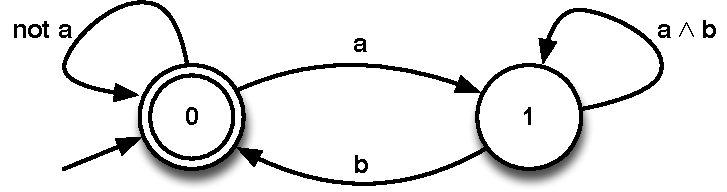
\includegraphics[width=.5\textwidth]{../images/future-slide} & 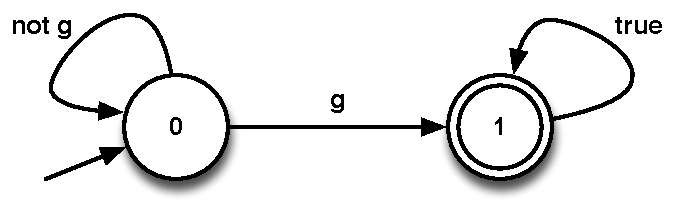
\includegraphics[width=.5\textwidth]{../images/past-slide}\\
%\end{tabular}\\
%\end{table}
%%\begin{figure}
%%\centering
%%\begin{subfigure}{0.5\textwidth}
%%  \centering
%% 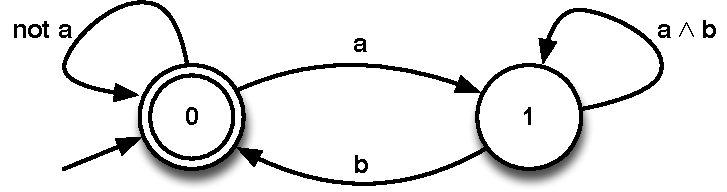
\includegraphics[]{../images/future-slide}
%%\end{subfigure}%
%%\begin{subfigure}{0.5\textwidth}
%%  \centering
%%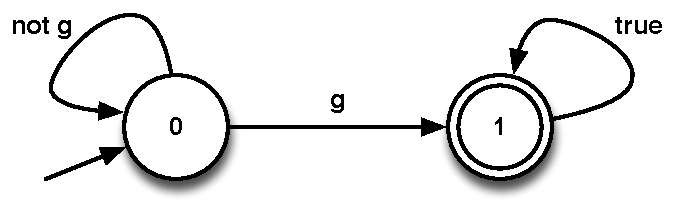
\includegraphics[]{../images/past-slide}
%%\end{subfigure}
%%\caption{A figure with two subfigures}
%%\label{fig:test}
%%\end{figure}
%\end{example}
	
	Output examples:
\begin{table}
	\centering
\begin{tabular}{c c} 
	$\varphi_1 = \Box(a \Rightarrow \Next b)$ & $\varphi_2 = \Once g$\\
    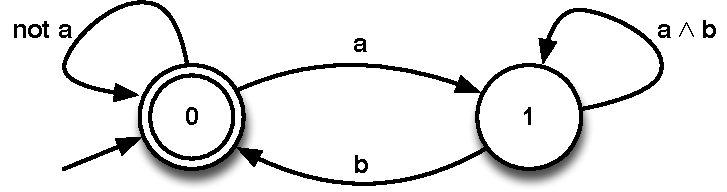
\includegraphics[width=.5\textwidth]{../images/future-slide} & 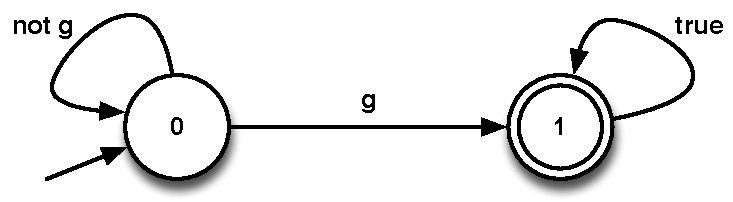
\includegraphics[width=.5\textwidth]{../images/future-pres}\\
%   	$\Box A$ & $\Diamond A$\\
%   	\emph{Always A} & \emph{Eventually A}\\ 
\end{tabular}\\
\end{table}
\end{frame}

\section{\FONDFOR}

\begin{frame}{\FOND Planning for Extended Temporal Goals}
\begin{itemize}
\item A \textit{fully observable non-deterministic} (\FOND) domain with initial state is a tuple $\D = \tup{2^\F, A, s_0, \varrho, \alpha}$, specified in \PDDL as domain $\D$ and problem $\P$

\item Actions effects are \emph{non-deterministic}: who chooses what?
\begin{itemize}
\item the \textcolor{blue}{Agent} chooses the \textcolor{blue}{action} to execute
\item the \textcolor{red}{Environment} chooses the \textcolor{red}{successor state}
\end{itemize}

\item Goals, planning and plans
\begin{itemize}
\item Goal: an \LTLf/\PLTL formula $\varphi$
\item Planning: a \emph{game} between the two players
\item Plan: \emph{strategy} to \emph{win} the game
\end{itemize}
\end{itemize}

\end{frame}

\begin{frame}{The \FONDFOR approach:}
%\fontsize{10}{9}\selectfont
\begin{itemize}
\item Idea: reduce the problem to standard \FOND planning
\item How to deal with \LTLf/\PLTL goal:
\begin{enumerate}
\item transform the goal $\varphi$ into the \DFA $\automaton_\varphi = \tup{\Sigma, Q, q_0 , \delta, F}$, through \LTLfToDFA
\item to capture the general representation of $\automaton_\varphi$ in the $\D$, we modify $\automaton_\varphi$ to $\automaton'_\varphi$
\begin{block}{\normalsize The parametrization of $\automaton_\varphi$: $\automaton'_\varphi$}
\begin{itemize}
\item $\Sigma = \{a_0(\vec{o}), \dots, a_n(\vec{o})\}$ to $\Sigma' = \{a'_0(\vec{x}), \dots, a'_n(\vec{x})\}$
\item $Q = \{q_0, \dots, q_n\}$ to $Q' = \{q'_0(\vec{x}), \dots, q'_n(\vec{x})\}$
\end{itemize}
where $\vec{o} = (o_0,\dots,o_k)$ and $\vec{x} = (x_0,\dots,x_k)$ 
\end{block}
\seti

\end{enumerate}
\end{itemize}


%\begin{block}{}
%Given a \PDDL domain $\D$, an initial state $s_0$ and a goal formula $\varphi$, we obtain $\automaton_\varphi = \tup{\Sigma, Q, q_0 , \delta, F}$ through \LTLfToDFA and we encode $\automaton_\varphi$ into $\D$
%\end{block}
%\begin{itemize}
%\item We perform an action on the domain and then update the automaton state. The \textit{turnDomain} predicate achieves this
%
%\item Encoding of automaton $\automaton_\varphi$ to \PDDL in domain $\D$:
%\begin{block}{Action \texttt{trans}}
%parameters: $(x_0, \dots, x_k)$, where $x_i \in \V$\\
%preconditions: $\lnot turnDomain$\\
%effects: $when\; (q_i(x_0, \dots, x_k) \lAND a'_j)\; then\; (\delta'(q'_i, a'_j)=q''_i(x_0, \dots, x_k) \lAND (\lnot q, \forall q \in Q \text{ s.t. } q \neq q''_i) \lAND turnDomain),\; \forall i,j: 0\leq i \leq m, 0\leq j \leq n$
%\end{block}
%
%\item New initial state: $s_0 \lAND \text{\texttt{turnDomain}} \lAND q_0(o_0,\dots,o_k)$
%%\item New goal specification: $\text{\texttt{turnDomain}} \lAND (\bigvee_{q \in F} q(o_0,\dots,o_k))$
%\end{itemize}

\end{frame}

\begin{frame}{}
%\begin{block}{}
%Given a \PDDL domain $\D$, an initial state $s_0$ and a goal formula $\varphi$, we obtain $\automaton_\varphi = \tup{\Sigma, Q, q_0 , \delta, F}$ through \LTLfToDFA and we encode $\automaton_\varphi$ into $\D$
%\end{block}
%\begin{itemize}
%\item We perform an action on the domain and then update the automaton state. The \textit{turnDomain} predicate achieves this
%
%\item Encoding of automaton $\automaton_\varphi$ to \PDDL in domain $\D$:
%\begin{block}{Action \texttt{trans}: encoding of $\delta'$ into domain $\D$}
%parameters: $(x_0, \dots, x_k)$, where $x_i \in \V$\\
%preconditions: $\lnot turnDomain$\\
%effects: $when\; (q_i(x_0, \dots, x_k) \lAND a'_j)\; then\; (\delta'(q'_i, a'_j)=q''_i(x_0, \dots, x_k) \lAND (\lnot q, \forall q \in Q \text{ s.t. } q \neq q''_i) \lAND turnDomain),\; \forall i,j: 0\leq i \leq m, 0\leq j \leq n$
%\end{block}

%\item New initial state: $s_0 \lAND \text{\texttt{turnDomain}} \lAND q_0(o_0,\dots,o_k)$
%\item New goal specification: $\text{\texttt{turnDomain}} \lAND (\bigvee_{q \in F} q(o_0,\dots,o_k))$
%\end{itemize}

\begin{enumerate}
\conti
\item introduce the \textit{turnDomain} predicate that enables to perform a step on the domain and another step on the \DFA alternatively
\item encode $\delta'$ of $\automaton'_\varphi$ in \PDDL:
\begin{block}{\normalsize Action \texttt{trans}: encoding of $\delta'$ into domain $\D$}
parameters: $(x_0, \dots, x_k)$, where $x_i \in \V$\\
preconditions: $\lnot turnDomain$\\
effects: $when\; (q_i(x_0, \dots, x_k) \lAND a'_j)\; then\; (\delta'(q'_i, a'_j)=q''_i(x_0, \dots, x_k) \lAND (\lnot q, \forall q \in Q \text{ s.t. } q \neq q''_i) \lAND turnDomain),\; \forall i,j: 0\leq i \leq m, 0\leq j \leq n$
\end{block}
\item in problem $\P$, produce a new initial state and new goal state accordingly
\begin{itemize}
\item New initial state: $s_0 \lAND \text{\texttt{turnDomain}} \lAND q_0(o_0,\dots,o_k)$
\item New goal specification: $\text{\texttt{turnDomain}} \lAND (\bigvee_{q \in F} q(o_0,\dots,o_k))$
\end{itemize}
\end{enumerate}
\end{frame}

\begin{frame}{Implementation and Results}
\begin{itemize}
\item \FONDFOR Python package using FOND-SAT planner
\item soon available online at \href{http://fond4ltlfpltl.diag.uniroma1.it}{http://fond4ltlfpltl.diag.uniroma1.it}
\end{itemize}

\begin{example}
Objective: Drive from one location to another. A tire may be going flat. If there is a spare tire in the location of the car, then the car can use it to fix the flat tire.

Goal: $\varphi = vehicleAt(l22) \lAND \Once (vehicleAt(l31))$

\textit{Strong Plan}: any path from state $0$ to state $5$ leads to the goal
\begin{figure}[h]
\centering
\subfigure{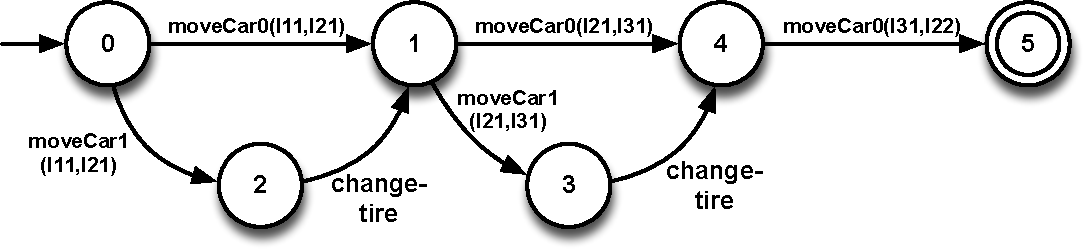
\includegraphics[width=.7\textwidth]{../images/result-plan-slide}}
\subfigure{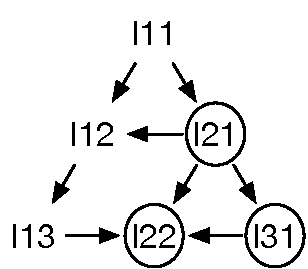
\includegraphics[width=.25\textwidth]{../images/plan-ex-slide}}
\end{figure}

%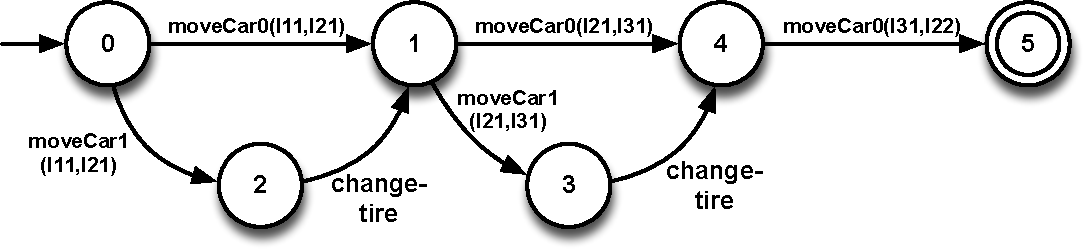
\includegraphics[width=.7\textwidth]{../images/result-plan-slide}
\end{example}

%\begin{figure}[h]
%\centering
%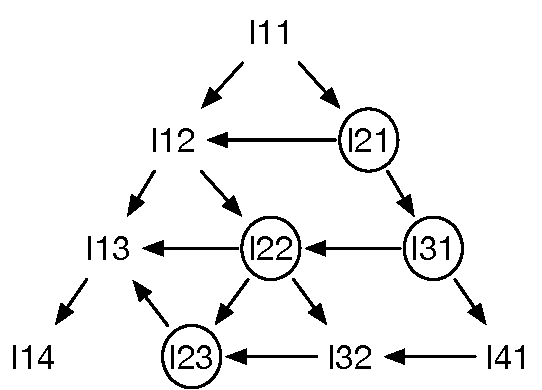
\includegraphics[width=0.5\textwidth]{../images/ttireworld-task}
%\caption{A possible Triangle Tireworld task. Locations marked with a circle have a spare tire, arrows represent possible directions} 
%\label{fig:ttireworld-task}
%\end{figure}

\end{frame}


\section{\janus}
\fontsize{10}{10}\selectfont
\begin{frame}{The Janus approach for Declarative Process Mining}
\begin{block}{}
Declarative Process Mining is the set of techniques aimed at determining if a trace $t$ is \emph{interesting} wrt a given temporal specification $\varphi$, called a constraint. 
\end{block}
\begin{itemize}
\item \textbf{Problem}: \emph{``ex falso quod libet''}, i.e. a constraint can be satisfied even though it is never activated
\item \textbf{Solution}: the Janus approach (Cecconi et al. 2018) proposed the \textit{reactive constraint} (\rcon\xspace) as $\Psi \doteq \alpha \mapsto \varphi$ where:
\begin{itemize}
\item $\alpha$ is the activation condition
\item $\varphi$ is an \LTLp formula (i.e. \LTLf augmented with \PLTL)
\end{itemize}
for computing the \emph{interestingness degree} function $\zeta(\Psi, t)$
\end{itemize}

\begin{exampleblock}{Example: $\Psi = a \mapsto (\Yesterday b \lOR \Diamond c)$}
Given a trace $t = \tup{d,f,a,f,c,a,f,b,a,f}$, the $\zeta(\Psi, t) = \tfrac{2}{3} = 0.667$
\end{exampleblock}

\begin{alertblock}{Two main drawbacks:}
$\alpha$ only a single task and implementation limited to \declare constraints
\end{alertblock}

\end{frame}

\begin{frame}
\fontsize{10}{9.2}\selectfont
Our generalization of the Janus approach extends the original approach:
\begin{block}{New constraint representation - \rcon\xspace}
\[\Psi \doteq \bigvee^{m}_{j=1} (\varphi^{\blacktriangleleft} \lAND \varphi^{\blacktriangledown} \lAND \varphi^{\blacktriangleright})_j\]
where $\varphi^{\blacktriangleleft}$ is a pure past formula, $\varphi^{\blacktriangledown}$ is a \textcolor{red}{propositional formula} on the current instant that triggers potential interest and $\varphi^{\blacktriangleright}$ is a pure future formula
\end{block}

\begin{block}{New \emph{interestingness degree} function $\eta(\Psi, t)$}
\[   
\eta(\Psi,t) = 
     \begin{cases}
       \dfrac{\lvert \{t \models \bigvee^{m}_{j=1} (\varphi^{\blacktriangleleft} \lAND \varphi^{\blacktriangledown} \lAND \varphi^{\blacktriangleright})_j\} \rvert}{\lvert \{t \models \bigvee^{m}_{j=1} \varphi^{\blacktriangledown}\} \rvert}, &\quad\text{if } \lvert \{t \models \bigvee^{m}_{j=1} \varphi^{\blacktriangledown}\} \rvert \neq 0 ;\\
       0, &\quad\text{otherwise} \\
     \end{cases}
\]
\end{block}

\begin{theorem}
The $\eta(\Psi, t)$ function is a generalization of the $\zeta(\Psi, t)$ function
\end{theorem}

\end{frame}

\begin{frame}{Implementation and Results}
\janus Python package:
	\begin{itemize}
		\item any type of constraint formula
		\item automata generation through \LTLfToDFA
	\end{itemize}
Results:
\begin{exampleblock}{Example taken from \textit{Sepsis}\footnotemark event log}
\begin{itemize}
\item Given an \rcon\xspace:
\begin{align*}
\Psi = \;& (\Yesterday ER\; Registration \lAND (Leucocytes \lAND LacticAcid) \lAND True) \lOR\\
& (True \lAND (Leucocytes \lAND LacticAcid) \lAND \Diamond CRP)
\end{align*}
\item $t$ = \{'ER Registration', ('ER Triage','ER Sepsis Triage), ('LacticAcid', 'IV Liquid'),  ('Leucocytes', 'LacticAcid'), 'CRP', 'LacticAcid', ('Leucocytes', 'LacticAcid'), ('Leucocytes', 'IV Antibiotics'),'IV Liquid', 'Release A'\}
\item $\eta(\Psi, t) = \tfrac{1}{2} = 0.5$
\end{itemize}
\end{exampleblock}
\footnotetext{\textit{Sepsis} reports trajectories of patients showing symptoms of sepsis in a Dutch hospital}
\end{frame}

\section{Conclusions}
\begin{frame}{Conclusions}
	\textbf{Thesis results}:
	\begin{itemize}
		\item Provided the \LTLfToDFA tool which implements the translation procedure from \LTLf/\PLTL to \DFA
		\item Proposed and implemented the \FONDFOR approach in compiling \LTLf/\PLTL goals along with the original planning domain, specified in \PDDL
		\item Extended the Janus approach both theoretically and practically
	\end{itemize}
	\vspace{0.5cm}
\textbf{Future works}:
	\begin{itemize}
		\item Investigate the \LTLp logic (i.e. \LTLf and \PLTL merged) for dealing directly with mixed formulas 
		\item Extend our research to \textit{Partially Observable Non Deterministic} (\POND) domains
		\item Provide a tool that automatically separates \LTLp formulas
		\item Optimize and enrich all tools developed.
	\end{itemize}
%Some of the topics described will be published
\end{frame}

%
%%\begin{block}{Examples}
%%Some examples of commonly used commands and features are included, to help you get started.
%%\end{block}
%
%
%
%%\section{Some \LaTeX{} Examples}
%
%%\subsection{Tables and Figures}
%
%\begin{frame}{Example of NMRDP: \Breakout}
%	\begin{itemize}
%		\item Non-Markovian reward: remove columns from left to right
%		\item The solution space is restricted
%		\item Policy must depend from a sequence of states: $\Policy: S^* \to A$
%	\end{itemize}
%
%%	\begin{figure}
%%		\centering
%%		\includegraphics[width=0.5\textwidth]{images/breakout.jpg}
%%	\end{figure}
%\end{frame}
%
%
%
%\begin{frame}{Goals of the thesis}
%
%\begin{itemize}
%\item Theoretical foundations for RL over NMRDP with \LLf rewards by leveraging (Brafman et al. 2018)
%
%\vskip 0.5cm
%
%\item Formalization and solution of a new problem: RL for \LLf goals 
%\begin{itemize}
%	\item two-fold representation of the world
%	\begin{itemize}
%		\item Low-level, used by the learning agent 
%		\item High-level, used to specify the goal formulas 
%	\end{itemize}
%
%
%\end{itemize}
%
%\vskip 0.5cm
%
%\item Deal with sparse rewards and design a way to improve exploration
%
%\vskip 0.5cm
%
%\item Implementation of the topics described above
%
%\end{itemize}
%
%\end{frame}
%
%%\subsection{Mathematics}
%
%\begin{frame}{\LTLf and \LDLf (De Giacomo and Vardi, 2013)}
%	\begin{itemize}
%		\item Linear Temporal Logic on finite traces: \LTLf
%			\begin{itemize}
%				\item Exactly the same syntax of \LTL
%				\item Interpreted over finite traces
%	
%			\begin{tasks}[counter-format = -](2)
%				\task Next: $\Next happy$
%				\task Until: $reply \lUntil acknowledge$
%				\task Eventually: $\Diamond rich$
%				\task Always: $\Box safe$
%			\end{tasks}
%%			\[\begin{array}{rcl}
%%			\varphi &::=& \Atom \mid \lnot \varphi \mid \varphi_1\land \varphi_2 \mid \Next\varphi \mid \varphi_1 \lUntil \varphi_2
%%			\end{array}
%%			\]
%			
%			\end{itemize}
%
%	
%		\item Linear Dynamic Logic on finite traces: \LTLf
%			\begin{itemize}
%				\item Merging of \LTLf and Regular Expressions
%	
%				\begin{tasks}[counter-format = -](2)
%					\task $\BOX{true^*}(safe)$
%					\task $\DIAM{A^*;B}End$
%				\end{tasks}
%%			\[\begin{array}{lcl}
%%			\varphi &::=& \ttrue  \mid \lnot \varphi \mid \varphi_1 \land \varphi_2 \mid \DIAM{\varrho}\varphi \\
%%			\varrho &::=& \phi \mid \varphi? \mid  \varrho_1 + \varrho_2 \mid \varrho_1; \varrho_2 \mid \varrho^*
%%			\end{array}
%%			\]
%			\end{itemize}
%		
%		\item Reasoning in \LLf:
%			\begin{itemize}
%				\item transform formulas $\varphi$ into NFAs or DFAs $\automaton_\varphi$
%				\item For every trace $\trace$ and \LLf formula $\varphi$: \[\trace \models \varphi \iff \trace \in \L(\automaton_\varphi)\]
%			\end{itemize}
%	\end{itemize}
%\end{frame}
%
%
%\begin{frame}{From \LLf formulas to automata: examples}
%E.g. For $\trace = \tup{\set{}, \set{A}, \set{A, B}}$, 
%\begin{table}
%	\centering
%\begin{tabular}{c c c} 
%	$\trace \not\models \Box A$ & $\trace \models \Diamond A$ & $\trace \not\models \DIAM{(A;B)^*}End$\\
%%    \includegraphics[width=.20\textwidth]{images/ltlf-alwaysA-dfa-no-borders} & \includegraphics[width=.20\textwidth]{images/ltlf-eventuallyA-dfa-no-borders} & \includegraphics[width=.35\textwidth]{images/alternating-sequence-dfa-no-borders} \\
%   	$\Box A$ & $\Diamond A$ & $\DIAM{(A;B)^*}End$ \\
%   	\emph{Always A} & \emph{Eventually A} & \emph{Alternating $A$ and $B$} \\ 
%\end{tabular}\\
%\end{table}
%
%
%% \begin{figure}
%% 	\centering
%% 	\subfloat[$\Box A$: “always A . Till the end of the trace, A holds”
%% 	\label{fig:a}]{\includegraphics[width=0.25\textwidth]{images/ltlf-alwaysA-dfa}}\qquad
%% 	\subfloat[$\Diamond A$: “Eventually A. Sooner or later, A holds”
%% 	\label{fig:b}]{\includegraphics[width=0.25\textwidth]{images/ltlf-eventuallyA-dfa}}\qquad
%% 	\subfloat[$\DIAM{(A;B)^*}End$: “Eventually A. Sooner or later, A holds”]{\includegraphics[width=0.25\textwidth]{images/alternating-sequence-dfa}}
%%% 	\caption{A figure}
%%% 	\label{fig:1}
%% \end{figure}
%%	
%\end{frame}
%
%\begin{frame}[fragile]{FLLOAT: From \LLf tO AutomaTa}
%
%\begin{itemize}
%	\item Python package supporting:
%	\begin{itemize}
%		\item \LLf formulas: parsing, syntax and semantics
%		\item Translation to automata (\NFA, \DFA, on-the-fly \DFA)
%	\end{itemize}
%
%		\item $\Box A$:
%\begin{lstlisting}[language=Python, style=Python, numbers=none]
%from flloat.parser.ltlf import LTLfParser
%parser = LTLfParser()
%always_A = parser("G(A)")
%dfa = always_A.to_automaton(determinize=True)
%dfa.to_dot("always_A.svg")
%\end{lstlisting}
%
%%					\begin{figure}
%%						\includegraphics[width=0.75\textwidth]{images/flloat-code-always-example}
%%					\end{figure}
%			\item $\DIAM{(A;B)^*}End$:
%\begin{lstlisting}[language=Python, style=Python, numbers=none]
%from flloat.parser.ldlf import LDLfParser
%parser = LDLfParser()
%alternating_AB = parser("<(A;B)*>end")
%dfa = alternating_AB.to_automaton(determinize=True)
%dfa.to_dot("alternating_AB.svg")
%\end{lstlisting}
%	\end{itemize}
%
%\end{frame}
%
%\begin{frame}{RL for NMRDP with \LLf rewards}
%	\begin{itemize}
%		\item Given an NMRDP $\NMRDP$ with:
%		\begin{itemize}
%			\item rewards specified by \LLf formulas 
%			\item over a set of propositional symbols $\Prop$
%			\item agent’s state space: $S \subseteq 2^\Prop$
%		\end{itemize}
%		\item 	We can transform it into an equivalent MDP $\MDP$ (Brafman et al. 2018)
%		\begin{itemize}
%			\item the state space of $\MDP$ is extended:\\
%					\[S' = S \times Q_1 \times \dots \times Q_m\]
%				where $Q_i$ is the set of states of $\automaton_{\varphi_i}$
%				
%			\item 	reward is given iff $q_i$ is an accepting state of $\automaton_{\varphi_i}$
%		\end{itemize}
%
%		\item An optimal policy for $\MDP$ is optimal for $\NMRDP$
%		\item We reduced RL for $\MDP$ to RL for $\NMRDP$
%
%		
%	\end{itemize}
%	
%	
%\end{frame}
%
%
%\begin{frame}{RL for \LLf goals: a new problem}
%	
%		\textbf{Two-fold representation} of the world $\W$:
%		\begin{itemize}
%			\item An agent learning an MDP with \textbf{\emph{low-level} features} $S$, trying to optimize reward $R$
%			\item \LLf goals $\set{(\varphi_i, r_i)_{i=1}^m}$ over a set of \textbf{\emph{high-level} features} $\F$, yielding a set of fluents configurations $\L = 2^\F$
%		\end{itemize}
%		
%		\textbf{Solution}: a non-Markovian policy $\Policy: S^*\to A$ that is optimal wrt rewards $r_i$ and $R$.
%		
%%		\begin{figure}
%%			\includegraphics[width=0.75\textwidth]{images/rl-two-representations-no-borders}
%%		\end{figure}
%		
%%		Notice: we have to deal with a joint transition model:
%%		\[Tr' = S \times \L \times A \to Prob(S, \L) \]
%			
%\end{frame}
%
%\begin{frame}
%	Our approach:
%	\begin{itemize}
%		\item Transform each $\varphi_i$ into \DFA $\automaton_{\varphi_i}$
%		\item Do RL over an MDP $\MDP'$ with a transformed state space:
%		\[S'= 
%		\tikz[baseline]{
%			\node[fill=yellow!20,anchor=base] (ts)
%			{$S$};
%		}
%		\times 
%		\tikz[baseline]{
%			\node[fill=blue!20,anchor=base] (tq)
%			{$Q_1 \times \dots \times Q_m$};
%		}
%		\]
%	\end{itemize}
%	
%%	\begin{tikzpicture}
%%	\end{tikzpicture}
%	
%%	\begin{tikzpicture}
%%	\node[anchor=south west,inner sep=0] at (0,0) {		\includegraphics[width=0.9\textwidth]{images/rl-two-representations-no-borders}};
%%%	\draw[red,ultra thick,rounded corners] (7.5,5.3) rectangle (9.4,6.2);
%%%	\node [draw=red, anchor=base] (sl) at (1.95,2.25) {};
%%	\node [anchor=base] (sl) at (1.95,2.3) {};
%%	\node [anchor=base] (ss) at (4.65, 3.8) {};
%%	\node [anchor=base] (sq) at (4.65, 2.5) {};
%%	\end{tikzpicture}
%	
%%	\begin{figure}
%%		\includegraphics[width=0.9\textwidth]{images/rl-two-representations-no-borders}
%%	\end{figure}
%		Notice: \textbf{the agent ignores the fluents} \tikz[baseline]{\node[fill=red!20,anchor=base] (tl) {$\L$}}!\\
%		
%		
%		The actual RL relies on standard RL algorithms (e.g. Sarsa($\lambda$))
%	
%	% Now it's time to draw some edges between the global nodes. Note that we
%	% have to apply the 'overlay' style.
%%	\begin{tikzpicture}[overlay]
%%	\path[->]<1-> (ts) edge [bend left] (ss);
%%	\path[->]<1-> (tq) edge [bend left] (sq);
%%	\path[->]<1-> (tl) edge [bend right] (sl);
%%	\end{tikzpicture}
%	
%\end{frame}
%
%\begin{frame}{Automata-based Reward Shaping}
%	\begin{itemize}
%		\item \emph{Reward sparsity} is the main issue: \textbf{Hard to learn complex behaviors without heuristics}
%	\end{itemize}
%
%	
%
%	
%	\textbf{Idea}: Give additional reward if, after a transition on $\automaton_\varphi$, we are closer to an accepting state (anticipate rewards)
%	
%	Based on \emph{Potential-Based Reward Shaping} (Ng et al., 1999):
%	\[F(s,a,s') = \DiscFact\Phi(s') - \Phi(s)\]
%	
%	Two modes:
%	\begin{itemize}
%		\item \emph{Off-line}: $\Phi(q)$ inversely proportional to the distance from any accepting state of $\automaton_\varphi$ 
%		\item \emph{On-line}: $\automaton_\varphi$ and $\Phi$ are built from scratch and updated while learning and discovering new states/transitions. Using \emph{Dynamic PBRS} (Devlin, 2012)
%	\end{itemize}
%	
%\end{frame}
%
%\begin{frame}[fragile]{RLTG (Reinforcement Learning for Temporal Goals)}
%	Reinforcement Learning Python framework that implements our approach
%	\begin{itemize}
%		\item Depends on \texttt{flloat} for the construction of $\automaton_{\varphi_i}$
%		\item Works also for classic RL
%		\item Highly customizable, uses OpenAI Gym interface
%	\end{itemize}
%	Example (in pseudocode):
%\begin{lstlisting}[language=Python, style=Python, numbers=none, escapechar = £]
%env = GymEnvironment()           # a Gym environment 
%agent = TGAgent(                 # the "temporal goal" agent
%    FeatureExtractor(...),       # generates the agent's space
%    Brain(...), #abstraction of RL algorithms (e.g. Sarsa)
%    [TemporalGoal(£$\varphi, r$£), ...] # list of temp. goal managers
%)
%trainer = TGTrainer(env, agent, stop_conditions=..., ...)
%trainer.main(...)                # starts the learning process
%
%\end{lstlisting}
%\end{frame}
%
%
%\begin{frame}{Experiments: \Breakout}
%\Breakout: remove columns/rows in a given order
%	\begin{itemize}
%		\item \textbf{low-level features}: paddle position, ball speed/position;
%		\item \textbf{high-level features}: bricks status (broken/not broken)
%		\item \textbf{\LLf goal} ($l_i$ means: the $i_{th}$ line has been removed.):
%		\[\DIAM{(\lnot l_0 \lAND \lnot l_1 \lAND \lnot l_2)^*;(l_0 \lAND \lnot l_1 \lAND \lnot l_2);(l_0 \lAND \lnot l_1 \lAND \lnot l_2)^*;\dots;(l_0 \lAND l_1 \lAND l_2)}tt\]
%	\end{itemize}
%	%\animategraphics[width=\textwidth]{12}{gifs/frame-}{0}{18}
%%	\begin{table}
%%		\centering
%%		\begin{tabular}{c c}
%%		 \includegraphics[width=.35\textwidth]{images/breakout.png} &
%%			\movie[height = 3.5cm, width = 4cm, showcontrols,	poster]{}{breakout-left-right.avi}
%%		\end{tabular}
%%	\end{table}
%
%	
%\end{frame}
%
%\begin{frame}{Experiments: \Sapientino}
%	\Sapientino: make a \emph{bip} in each color, in a given order
%	\begin{itemize}
%		\item \textbf{low-level features}: robot position $(x, y)$;
%		\item \textbf{high-level features}: color of current cell, bip-last-action
%		\item \textbf{\LLf goal}:
%		\[\DIAM{(¬bip)^* ;red \wedge bip; (¬bip)^*;green \wedge bip; \dots}tt\]
%	\end{itemize}
%	
%	%\animategraphics[width=\textwidth]{12}{gifs/frame-}{0}{18}
%%	\begin{table}
%%		\centering
%%		\includegraphics[width=0.6\textwidth]{images/sapientino_ldlf_horizontal}
%%		\begin{tabular}{c}
%%			\movie[height = 3.7cm, width = 4cm, showcontrols,	poster]{}{sapientino.avi}
%%		\end{tabular}
%%	\end{table}
%
%\end{frame}
%
%\begin{frame}{Experiments: \Minecraft}
%	\Minecraft: complete tasks by getting resources/using tools
%	\begin{itemize}
%		\item \textbf{low-level features}: robot position $(x, y)$;
%		\item \textbf{high-level features}: $get\_wood$, $use\_workbench$ etc.
%		\item \textbf{\LLf goal}: three composite tasks like (approximately):
%		\[
%		\DIAM{\true^*}\DIAM{get\_iron ; get\_iron \lAND get\_wood; \dots \lAND use\_factory}tt
%		\]
%	\end{itemize}
%	
%	%\animategraphics[width=\textwidth]{12}{gifs/frame-}{0}{18}
%%	\begin{table}
%%		\centering
%%		\begin{tabular}{c c}
%%			\includegraphics[width=0.3\textwidth]{images/minecraft_goals_no_borders} &
%%			\movie[height = 3.7cm, width = 4cm, showcontrols,	poster]{}{minecraft.avi}
%%		\end{tabular}
%%	\end{table}
%	
%\end{frame}
%
%
%
%\begin{frame}{Discussion}
%
%	Why a two-fold representation for temporal goals?
%	\begin{itemize}
%		\item \emph{Separation of concerns}: It allows to a better design of the RL system by improving modularity and flexibility;
%		\item \emph{Reduced state space}: It makes easier the learning by exploring a smaller state space and focusing only on relevant low-level features;
%		\item \emph{Simpler agent}: Move part of the complexity outside the agent.
%	\end{itemize}
%	Other observations:
%	\begin{itemize}
%		\item \emph{Expressive Power}: \LDLf expressive as Monadic Second-Order logic (e.g. we can specify procedural constraints);
%		\item No need of new algorithms, one can rely on off-the-shelf RL algorithms (Sarsa($\lambda$), Q-Learning, ...);
%		\item The correlation between the two representations does not need to be formalized.
%	\end{itemize}
%
%\end{frame}
%
%\begin{frame}{Conclusions}
%	Thesis results:
%	\begin{itemize}
%		\item Extended (Brafman et al. 2018) to the context of RL;
%		\item Formalization of \emph{RL for \LLf goals}, devising of a solution and analysis of the advantages;
%		\item Provided an implementation and given experimental evidence of the goodness of our approach.
%	\end{itemize}
%	Future works:
%	\begin{itemize}
%		\item Minimal low-level representation to tackle \LLf goals;
%		\item Optimize FLLOAT, enrich RLTG;
%		\item Try the approach in several real world applications;
%		\item Design of ad-hoc algorithms (e.g. "automata-aware" exploration);
%		\item Extend the approach to the framework of Multi-Agent Systems.
%	\end{itemize}
%	Publication: \href{https://arxiv.org/abs/1807.06333}{https://arxiv.org/abs/1807.06333}. Status: submitted
%	
%\end{frame}

\end{document}
